% =====================================================================
%  Laboratory report 1 -- Biosignal Processing (English version)
%  Hardware setup & data acquisition
%
%  English translation of laborbericht.tex (MCI LaTeX template V3.0):
%  same document class, % =====================================================================
%  definitions.tex -- angepasste Kopie von Vorlagen/definitions.tex
%  (MCI-Vorlage V3.0, Drauschke/Teschl/Mehrle)
%
%  Layout, Farben, Überschriften, Abstände und Verzeichnisnamen sind
%  unverändert übernommen. Geändert wurde nur, was mit pdflatex /
%  aktuellem TeX Live nicht mehr kompiliert:
%    - "german"           -> babel/ngerman + UTF-8 (Umlaute direkt tippen)
%    - graphicx[dvips]    -> graphicx (pdflatex kann PNG/PDF einbinden)
%    - pst-all, wallpaper, pgfplots, units, subfigure entfernt
%      (Konflikte \unit/\ang, nur für latex+dvips gedacht, nicht benötigt)
%    - PSTricks-Makros (Netzwerk-/Blocksymbole) entfernt
%  Ergänzt: booktabs, listings, \todo für offene Stellen.
% =====================================================================

\ifthenelse{\boolean{english}}
  {\usepackage[english]{babel}}
  {\usepackage[ngerman]{babel}}
\usepackage[utf8]{inputenc}
\usepackage[T1]{fontenc}
\usepackage{lmodern}
\usepackage{graphicx}
\usepackage[tmargin=1in,bmargin=1in,lmargin=1.25in,rmargin=1.25in]{geometry}
\usepackage{titlesec}
\usepackage{xcolor}
\usepackage[overload]{textcase}
\definecolor{MSBlue}{rgb}{.204,.353,.541}
\definecolor{MSLightBlue}{rgb}{.31,.506,.741}
% Set formats for each heading level (Abschnitte klein geschrieben wie in der Vorlage)
\titleformat{\section}[hang]{\rmfamily\bfseries\huge\color{MSBlue}}{\thesection}{1em}{\MakeLowercase}[]
\titleformat{\subsection}{\large\bfseries\sffamily\uppercase}{\thesubsection}{1em}{}
\titleformat{\subsubsection}{\sffamily\bfseries}{\thesubsubsection}{1em}{}
% babel überschreibt die Namen bei \begin{document}, daher erst dort setzen
% (\ifthenelse außerhalb, weil \MakeLowercase es in der Überschrift nicht verträgt)
\ifthenelse{\boolean{english}}
  {\AtBeginDocument{%
    \renewcommand\contentsname{table of contents.}%
    \renewcommand\listfigurename{list of figures.}%
    \renewcommand\listtablename{list of tables.}%
    \renewcommand\refname{\litname.}}}
  {\AtBeginDocument{%
    \renewcommand\contentsname{inhaltsverzeichnis.}%
    \renewcommand\listfigurename{abbildungsverzeichnis.}%
    \renewcommand\listtablename{tabellenverzeichnis.}%
    \renewcommand\refname{\litname.}}}
\usepackage{exscale,relsize}
\usepackage{fancyhdr}
\usepackage[small]{caption}
\usepackage{float}
\usepackage{amsmath}
\usepackage{amssymb}
\usepackage{rotating}
\usepackage{mathrsfs}
\usepackage{booktabs}
\usepackage{listings}
\setlength{\emergencystretch}{2em}

\newcommand{\babel}[2]{\ifthenelse{\boolean{english}}{#1}{#2}}

% auxillary symbols
\newcommand{\define}{\stackrel{!}{=}}
\renewcommand{\equiv}{\,\widehat{=}\,}
\newcommand{\subsubsubsection}{\textbf}
\newcommand{\mif}{\quad\mathrm{\babel{if}{falls}}\quad}
\newcommand{\with}{\quad\mathrm{\babel{with}{mit}}\quad}
\newcommand{\for}{\quad\mathrm{\babel{for}{für}}\quad}
\newcommand{\matlab}{MATLAB}

% format specifications
\renewcommand{\emph}{\textbf}
\newcommand{\file}{\textit}
\newcommand{\cmd}{\texttt}
\newcommand{\ten}{\boldsymbol}
\newcommand{\lemma}{\textit}

% Pfade zu Grafiken
\graphicspath{{abbildungen/}{../Abgabe_Lab1/figures/}}

% mathematical operators
\newcommand{\grad}{\,\mathrm{grad}\,}
\renewcommand{\div}{\,\mathrm{div}\,}
\newcommand{\rot}{\,\mathrm{rot}\,}
\newcommand{\lap}{\Delta}
\newcommand{\laplace}[1]{\mathscr{L}\left\{#1\right\}}
\newcommand{\trans}{^T}

\setlength{\parindent}{0em}
\setlength{\parskip}{1.5ex plus0.5ex minus0.5ex}
\setlength{\captionmargin}{3em}

% Quellcode (für Ausschnitte und Anhang)
\lstset{basicstyle=\ttfamily\footnotesize,frame=single,columns=fullflexible,
        keywordstyle=\bfseries,language=C++,breaklines=true}

% Offene Stellen rot markieren -- vor der Abgabe müssen alle weg sein
\newcommand{\todo}[1]{\textcolor{red}{\textbf{[TODO:} #1\textbf{]}}}
 and % Deckblatt:
\thispagestyle{empty}
\sffamily
%\put(-30,-685){\includegraphics[width=1.15\linewidth]{BG}}

{\bfseries


\vspace*{1cm}

\def\thesis{\ifthenelse{\boolean{english}}{laboratory report}{laborbericht}}
\textcolor{MSBlue}{\rmfamily\bfseries\huge\thesis.}%

\vspace*{0.5cm}

\textbf{\labtitle{ }(\labcode)}

\labname

\ifthenelse{\boolean{english}}{Lab}{Labor} \labnum

\vspace*{10cm}

\textcolor{gray}{\study}

\def\termname{\ifthenelse{\boolean{english}}{semester}{Semester}}
\textcolor{gray}{\term{ }\termname}

\def\lecturername{\ifthenelse{\boolean{english}}{Responsible lecturer}{Lehrveranstaltungsleiter}}
\textcolor{gray}{\lecturername: \lecturer}

\def\groupname{\ifthenelse{\boolean{english}}{Group}{Jahrgang}}
\textcolor{gray}{\groupname: \group}

\def\authorname{\ifthenelse{\boolean{english}}{Author}{Verfasser}}
\textcolor{gray}{\authorname: \student}

\textcolor{gray}{\today}

\newpage}
,
%  same structure. The boolean "english" switches babel, the cover page
%  and the directory names to English.
%
%  The references are given inline (thebibliography, formatted as by
%  IEEEtran from Literatur.bib) so that the notes of the shared
%  Literatur.bib ("Datenblatt", "heute NXP") appear in English without
%  changing the German version.
%
%  Compile:  latexmk -pdf laborbericht_en.tex
%  Max. 10 pages (incl. cover page).
% =====================================================================

\documentclass[a4paper,oneside,10pt]{article}

\usepackage{ifthen}
\newboolean{english}
\setboolean{english}{true}		% comment out for the German version

% =====================================================================
%  definitions.tex -- angepasste Kopie von Vorlagen/definitions.tex
%  (MCI-Vorlage V3.0, Drauschke/Teschl/Mehrle)
%
%  Layout, Farben, Überschriften, Abstände und Verzeichnisnamen sind
%  unverändert übernommen. Geändert wurde nur, was mit pdflatex /
%  aktuellem TeX Live nicht mehr kompiliert:
%    - "german"           -> babel/ngerman + UTF-8 (Umlaute direkt tippen)
%    - graphicx[dvips]    -> graphicx (pdflatex kann PNG/PDF einbinden)
%    - pst-all, wallpaper, pgfplots, units, subfigure entfernt
%      (Konflikte \unit/\ang, nur für latex+dvips gedacht, nicht benötigt)
%    - PSTricks-Makros (Netzwerk-/Blocksymbole) entfernt
%  Ergänzt: booktabs, listings, \todo für offene Stellen.
% =====================================================================

\ifthenelse{\boolean{english}}
  {\usepackage[english]{babel}}
  {\usepackage[ngerman]{babel}}
\usepackage[utf8]{inputenc}
\usepackage[T1]{fontenc}
\usepackage{lmodern}
\usepackage{graphicx}
\usepackage[tmargin=1in,bmargin=1in,lmargin=1.25in,rmargin=1.25in]{geometry}
\usepackage{titlesec}
\usepackage{xcolor}
\usepackage[overload]{textcase}
\definecolor{MSBlue}{rgb}{.204,.353,.541}
\definecolor{MSLightBlue}{rgb}{.31,.506,.741}
% Set formats for each heading level (Abschnitte klein geschrieben wie in der Vorlage)
\titleformat{\section}[hang]{\rmfamily\bfseries\huge\color{MSBlue}}{\thesection}{1em}{\MakeLowercase}[]
\titleformat{\subsection}{\large\bfseries\sffamily\uppercase}{\thesubsection}{1em}{}
\titleformat{\subsubsection}{\sffamily\bfseries}{\thesubsubsection}{1em}{}
% babel überschreibt die Namen bei \begin{document}, daher erst dort setzen
% (\ifthenelse außerhalb, weil \MakeLowercase es in der Überschrift nicht verträgt)
\ifthenelse{\boolean{english}}
  {\AtBeginDocument{%
    \renewcommand\contentsname{table of contents.}%
    \renewcommand\listfigurename{list of figures.}%
    \renewcommand\listtablename{list of tables.}%
    \renewcommand\refname{\litname.}}}
  {\AtBeginDocument{%
    \renewcommand\contentsname{inhaltsverzeichnis.}%
    \renewcommand\listfigurename{abbildungsverzeichnis.}%
    \renewcommand\listtablename{tabellenverzeichnis.}%
    \renewcommand\refname{\litname.}}}
\usepackage{exscale,relsize}
\usepackage{fancyhdr}
\usepackage[small]{caption}
\usepackage{float}
\usepackage{amsmath}
\usepackage{amssymb}
\usepackage{rotating}
\usepackage{mathrsfs}
\usepackage{booktabs}
\usepackage{listings}
\setlength{\emergencystretch}{2em}

\newcommand{\babel}[2]{\ifthenelse{\boolean{english}}{#1}{#2}}

% auxillary symbols
\newcommand{\define}{\stackrel{!}{=}}
\renewcommand{\equiv}{\,\widehat{=}\,}
\newcommand{\subsubsubsection}{\textbf}
\newcommand{\mif}{\quad\mathrm{\babel{if}{falls}}\quad}
\newcommand{\with}{\quad\mathrm{\babel{with}{mit}}\quad}
\newcommand{\for}{\quad\mathrm{\babel{for}{für}}\quad}
\newcommand{\matlab}{MATLAB}

% format specifications
\renewcommand{\emph}{\textbf}
\newcommand{\file}{\textit}
\newcommand{\cmd}{\texttt}
\newcommand{\ten}{\boldsymbol}
\newcommand{\lemma}{\textit}

% Pfade zu Grafiken
\graphicspath{{abbildungen/}{../Abgabe_Lab1/figures/}}

% mathematical operators
\newcommand{\grad}{\,\mathrm{grad}\,}
\renewcommand{\div}{\,\mathrm{div}\,}
\newcommand{\rot}{\,\mathrm{rot}\,}
\newcommand{\lap}{\Delta}
\newcommand{\laplace}[1]{\mathscr{L}\left\{#1\right\}}
\newcommand{\trans}{^T}

\setlength{\parindent}{0em}
\setlength{\parskip}{1.5ex plus0.5ex minus0.5ex}
\setlength{\captionmargin}{3em}

% Quellcode (für Ausschnitte und Anhang)
\lstset{basicstyle=\ttfamily\footnotesize,frame=single,columns=fullflexible,
        keywordstyle=\bfseries,language=C++,breaklines=true}

% Offene Stellen rot markieren -- vor der Abgabe müssen alle weg sein
\newcommand{\todo}[1]{\textcolor{red}{\textbf{[TODO:} #1\textbf{]}}}


\def\labtitle{Biosignal Processing}
\def\labcode{BA-MGST-B-3-BB-BS-ILV}
\def\labname{Hardware Setup \& Data Acquisition -- Group 4}
\def\labnum{1}

\def\study{Bachelor Medical, Sports and Health Technology}
\def\term{3rd}
\def\lecturer{Aitor Morillo}
\def\group{MGST-25}
\def\student{Matthias Zoller, Laurenz Keller, Matteo Harrasser}

\def\litname{references}

\begin{document}

% initialise header and footer
\pagestyle{plain}

% Deckblatt:
\thispagestyle{empty}
\sffamily
%\put(-30,-685){\includegraphics[width=1.15\linewidth]{BG}}

{\bfseries


\vspace*{1cm}

\def\thesis{\ifthenelse{\boolean{english}}{laboratory report}{laborbericht}}
\textcolor{MSBlue}{\rmfamily\bfseries\huge\thesis.}%

\vspace*{0.5cm}

\textbf{\labtitle{ }(\labcode)}

\labname

\ifthenelse{\boolean{english}}{Lab}{Labor} \labnum

\vspace*{10cm}

\textcolor{gray}{\study}

\def\termname{\ifthenelse{\boolean{english}}{semester}{Semester}}
\textcolor{gray}{\term{ }\termname}

\def\lecturername{\ifthenelse{\boolean{english}}{Responsible lecturer}{Lehrveranstaltungsleiter}}
\textcolor{gray}{\lecturername: \lecturer}

\def\groupname{\ifthenelse{\boolean{english}}{Group}{Jahrgang}}
\textcolor{gray}{\groupname: \group}

\def\authorname{\ifthenelse{\boolean{english}}{Author}{Verfasser}}
\textcolor{gray}{\authorname: \student}

\textcolor{gray}{\today}

\newpage}


\tableofcontents
\listoffigures
% \listoftables   % removed due to the 10-page limit

\newpage

% initialise header and footer
\pagestyle{fancy}

% =====================================================================
\section{Introduction}
% =====================================================================
The aim of the first lab is to set up a measurement system for acquiring
acceleration data and to process these data in Python. For this purpose, the
3-axis accelerometer BMA400 is connected via I\textsuperscript{2}C to an
Arduino (SparkFun RedBoard Qwiic); the data are transmitted to a PC via the serial
interface and then imported, filtered and plotted in Python.
In particular, we investigate the influence of the sensor's output data rate (ODR) on
the quality of the measured data, the sampling frequency actually achieved, and the
difference between a stationary (USB) and a mobile (data logger, battery)
measurement system.

% =====================================================================
\section{Experimental Setup}
% =====================================================================

\subsection{Stationary Measurement System (Task 1)}

Figure~\ref{fig:messsystem} shows the stationary measurement system with all
components, buses and signal paths.

\begin{figure}[H]
    \centering
    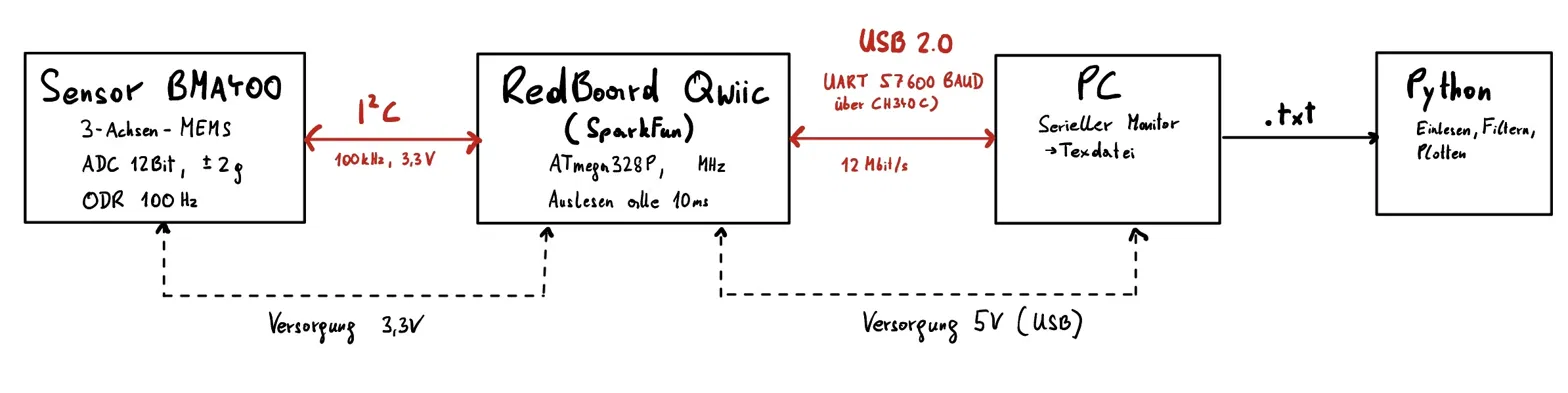
\includegraphics[width=\textwidth]{Messchaltung.png}
    \caption{Setup of the stationary measurement system (own illustration). Red: buses with type and speed, black: data path to Python, dashed: power supply.}
    \label{fig:messsystem}
\end{figure}

\textbf{Components:}
\begin{description}
    \item[BMA400 (SparkFun breakout \cite{sparkfun}):] Digital 3-axis MEMS accelerometer with
    12-bit resolution. Measurement range ($\pm 2$ to $\pm 16\,g$) and output data rate (ODR, 12.5--800\,Hz)
    are configurable; the measured values are stored in registers 0x04--0x09 \cite{bma400}.
    \item[SparkFun RedBoard Qwiic (ATmega328P, 16\,MHz, Arduino Uno compatible):] Configures the sensor, reads the six
    data registers, converts the raw values to $g$ and appends the time stamp
    \texttt{millis()}. It supplies the sensor with 3.3\,V.
    \item[PC (Arduino IDE):] The serial monitor displays the measured values line by line
    (\texttt{X Y Z Time}); they are copied and pasted into a \texttt{.txt} file.
    \item[Python (\texttt{MainCode1.ipynb}):] Reads the text file with \texttt{pandas},
    filters with \texttt{SciPy} \cite{scipy} and plots the data with \texttt{matplotlib}.
\end{description}

\textbf{Buses and signal paths:}
\begin{description}
    \item[I\textsuperscript{2}C (100\,kHz):] Two-wire bus (SDA = A4, SCL = A5). The Arduino is
    the master, the sensor the slave with address 0x14.
    \item[UART / USB 2.0:] The Arduino transmits serially at 57\,600\,baud; the USB-to-serial converter
    CH340C on the board converts this to USB 2.0 Full Speed (12\,Mbit/s).
    \item[Data path PC $\rightarrow$ Python:] Transfer of the measured data as a text file.
    \item[Power supply:] 5\,V via USB for the Arduino, 3.3\,V and GND from the Arduino
    to the sensor.
\end{description}

\subsection{Mobile Measurement System}

For Task~9, the USB connection is replaced by a data logger and a battery.
According to \texttt{Lab1Code2}, the mobile system consists of the Arduino, the
accelerometer \textbf{MMA8452Q} (SparkFun, $\pm 8\,g$, ODR 200\,Hz) and
a \textbf{Qwiic OpenLog} (SparkFun) with a microSD card. Sensor and OpenLog are
both connected to the Arduino's I\textsuperscript{2}C bus (OpenLog address 42); the Arduino
sends each measurement line via I\textsuperscript{2}C to the OpenLog, which writes it to the file
\texttt{ACCdata.txt} on the SD card. The file is then evaluated on the PC.
Instead of USB, power is supplied by a 9\,V alkaline battery
(6LR61 block battery); the Arduino's voltage regulator derives 5\,V and 3.3\,V from it.

% =====================================================================
\section{Preliminary Work}
% =====================================================================

\subsection{Measurement Strategy}

\begin{itemize}
  \item \textbf{Dynamic measurement:} fast up-and-down movement (approx.\ 1\,Hz), first with
        the original code (ODR 12.5\,Hz), then with increased ODR (Tasks 4 and 5).
  \item \textbf{Static measurement:} hold the sensor still in each of the six orientations for
        approx.\ 10\,s to check axis assignment, sign and magnitude ($\approx 1\,g$)
        (Task 6).
  \item \textbf{Time base:} time stamp \texttt{millis()} directly on the Arduino, used to
        determine the actual sampling frequency (Tasks 8 and 9).
\end{itemize}

\subsection{Conversion of an ADC Value into a Temperature (Task 2)}

Given are a temperature sensor with $U = 0 \ldots 3.3$\,V for
$\vartheta = 0 \ldots 40\,^\circ$C (linear) and an ADC with $n = 10$\,bit
($0 \ldots 1023$) and reference voltage $U_\mathrm{ref} = 5$\,V. The ADC returns
$D = 520$.

\textbf{Step 1 -- ADC value to voltage:}
\begin{equation}
  U = \frac{D}{2^{n}-1}\cdot U_\mathrm{ref} = \frac{520}{1023}\cdot 5\,\mathrm{V} \approx 2.542\,\mathrm{V}
\end{equation}

\textbf{Step 2 -- Voltage to temperature:}
\begin{equation}
  \vartheta = \frac{U}{3.3\,\mathrm{V}}\cdot 40\,^\circ\mathrm{C}
            = \frac{2.542\,\mathrm{V}}{3.3\,\mathrm{V}}\cdot 40\,^\circ\mathrm{C}
            \approx \mathbf{30.8\,^\circ C}
\end{equation}

The sensor thus measures approx.\ 30.8\,°C, which is plausible for a measurement on the skin
(skin temperature is below the core body temperature of approx.\ 37\,°C).
Since the sensor delivers at most 3.3\,V, only ADC values up to
$\frac{3.3}{5}\cdot 1023 \approx 675$ are used; the resolution is therefore
$40\,^\circ\mathrm{C}/675 \approx 0.06\,^\circ$C per step instead of the possible
$0.04\,^\circ$C.

\subsection{Axis Assignment and Conversion into Physical Quantities (Task 3)}

\textbf{Axis assignment:} \texttt{Lab1Code1} outputs \texttt{X Y Z Time} per line;
the columns follow the order of the data registers (0x04/0x05 = $x$,
0x06/0x07 = $y$, 0x08/0x09 = $z$) and thus the axes printed on the board.

\textbf{Test:} The sensor is placed so that one axis points vertically upwards.
This axis then reads approx.\ $+1\,g$, the others approx.\ $0\,g$. Lying flat on the
table ($z$ upwards), e.\,g.\ \texttt{7 -91 1002} was measured, i.\,e.\ $z \approx 1\,g$.
All six orientations are checked systematically in Task~6.

\textbf{Unit:} The output consists of raw values in LSB (digits): two registers per axis
(LSB, MSB), which together form a 12-bit value in two's complement
($-2048 \ldots +2047$):
\texttt{raw = ((msb \& 0x0F) << 8) | lsb}, then if \texttt{raw > 2047}
$\rightarrow$ \texttt{raw -= 4096}.

\textbf{Conversion:} According to the data sheet \cite{bma400} (p.~10, table \emph{Output Signal}), the sensitivity is
$S = 2048/\text{range}$, i.\,e.\ $S = 1024$\,LSB/$g$ at $\pm 2\,g$:
\begin{equation}
  a\,[g] = \frac{\text{raw}}{1024}, \qquad
  a\,[\mathrm{m/s^2}] = \frac{\text{raw}}{1024}\cdot 9.81\,\mathrm{m/s^2}
\end{equation}
Example: $1002/1024 = 0.98\,g = 9.60$\,m/s$^2$.

\subsection{Scripts}

The Python code \texttt{MainCode1.ipynb} covers Tasks 4\,(a), 5,
6\,(a), 7, 8 and 9 and generates all figures in this report. The Arduino code
was adapted for Task~5 (\texttt{Lab1Code1\_modifiziert.ino}). Both files
are included in the submission (Appendix~\ref{sec:anhang}).

% =====================================================================
\section{Results}
% =====================================================================

\subsection{Up-and-Down Movement with the Original Code (Task 4)}

The sensor was moved without rotation, and the data were recorded with \texttt{Lab1Code1}
(ODR 12.5\,Hz, $\pm 2\,g$) and copied into a text file.

\textbf{(a)} Figure~\ref{fig:a4} shows 4\,s of the measurement, converted to $g$.

\begin{figure}[H]
  \centering
  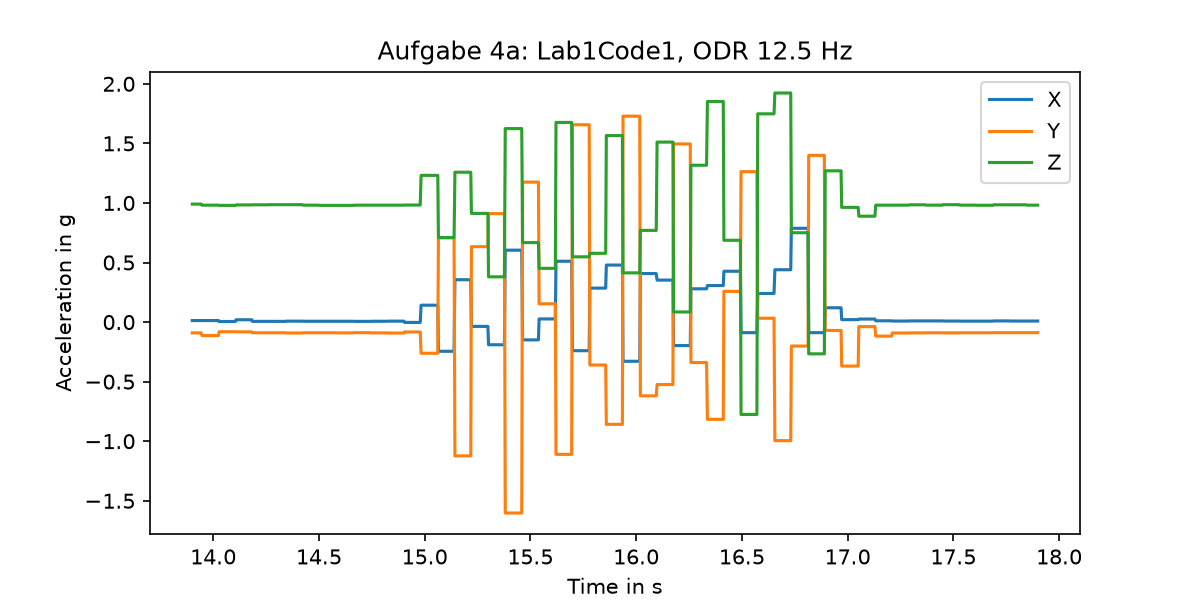
\includegraphics[width=0.85\textwidth]{A4a_12_5Hz.png}
  \caption{Up-and-down movement with \texttt{Lab1Code1} (ODR 12.5\,Hz), 4\,s excerpt.}
  \label{fig:a4}
\end{figure}

\textbf{(b) Plateaus of the peaks:} Each value remains constant for approx.\ 80\,ms, which
produces the step-like plateaus. The sensor only provides new values at the
ODR of 12.5\,Hz (every 80\,ms), but without a \texttt{delay} the \texttt{loop()}
outputs a line approx.\ every 3\,ms ($\approx 313$\,Hz, cf.\ Tab.~\ref{tab:fs}).
Until a new value is available in the data register, the same value is therefore read
again and again (approx.\ 25 identical lines per sample). \textbf{Solution:} Increase the ODR in
register \texttt{ACC\_CONFIG1} (Task~5) and match the output rate to the ODR with a
suitable \texttt{delay}. In addition, the peaks in $z$
(incl.\ gravity) of approx.\ $1.9\,g$ are close to the range limit of
$\pm 2\,g$; for stronger movements the measurement range should therefore also be increased
to avoid saturation.

\textbf{(c) Deviation from the actual movement:} At 12.5\,Hz, the
Nyquist frequency is 6.25\,Hz. The fast movement contains higher
frequency components, so that \emph{aliasing} occurs: there are only a few
samples per movement, and the signal (especially in $y$) changes sign at almost every sample
instead of showing the course of the movement. Moreover, the sensor always measures
gravity as well; if the hand rotates slightly, it is distributed across
several axes.

\subsection{Adjustment of the Sensor Configuration (Task 5)}

The new measurement was performed with the MMA8452Q accelerometer, for which
\texttt{Lab1Code1} was originally written (range $\pm 2\,g$, data rate
1.56\,Hz). According to the MMA8452Q data sheet \cite{mma8452q}, the data rate is set in register
\texttt{CTRL\_REG1} (0x2A) via the parameter \texttt{DR[2:0]} (bits 5:3)
(p.~37, Tab.~53 and 55). The possible values are listed in Tab.~\ref{tab:odr}.
In addition, the measurement range was changed in register \texttt{XYZ\_DATA\_CFG} (0x0E) via
\texttt{FS[1:0]} (bits 1:0) (p.~22, Tab.~15 and 16): 00 = $\pm 2\,g$, 01 = $\pm 4\,g$,
10 = $\pm 8\,g$, 11 = reserved.

\begin{table}[H]
\centering
\small
\caption{Possible values of the parameter \texttt{DR[2:0]} in register \texttt{CTRL\_REG1} (0x2A) of the MMA8452Q.}
\label{tab:odr}
\begin{tabular}{lcccccccc}
\toprule
\texttt{DR[2:0]} & 000 & 001 & 010 & \textbf{011} & 100 & 101 & 110 & 111 \\
\midrule
ODR / Hz & 800 & 400 & 200 & \textbf{100} & 50 & 12.5 & 6.25 & 1.56 \\
\bottomrule
\end{tabular}
\end{table}

The following lines were changed in the code (\texttt{Lab1Code1\_modifiziert.ino}):
\begin{lstlisting}
accel.setScale(SCALE_8G);     // XYZ_DATA_CFG (0x0E), FS = 10, previously SCALE_2G
accel.setDataRate(ODR_100);   // CTRL_REG1 (0x2A), DR = 011, previously ODR_1 (1.56 Hz)
\end{lstlisting}
In \texttt{loop()}, output only occurs when the sensor has a new value
(\texttt{accel.available()}). The raw values are converted to $g$ in Python with 256\,LSB/$g$
(12\,bit at $\pm 8\,g$).

\textbf{Justification:} Hand movements are well below 50\,Hz (Nyquist frequency
at 100\,Hz) and are therefore captured without aliasing. Higher rates are not necessary
and only load the transmission: one output line (e.\,g.\
\texttt{-23\textbackslash t3\textbackslash t-252\textbackslash t41000}
+ line break) comprises approx.\ 20 characters $\approx 200$\,bit, so at 57\,600\,baud
only approx.\ 290 lines/s can be transmitted -- from 400\,Hz on, the serial interface would be
overloaded. The range of $\pm 8\,g$ prevents fast movements above
$2\,g$ from being clipped (saturation); in return, the resolution drops to
$1/256\,g \approx 4\,mg$, which is sufficient for hand movements.

\begin{figure}[H]
  \centering
  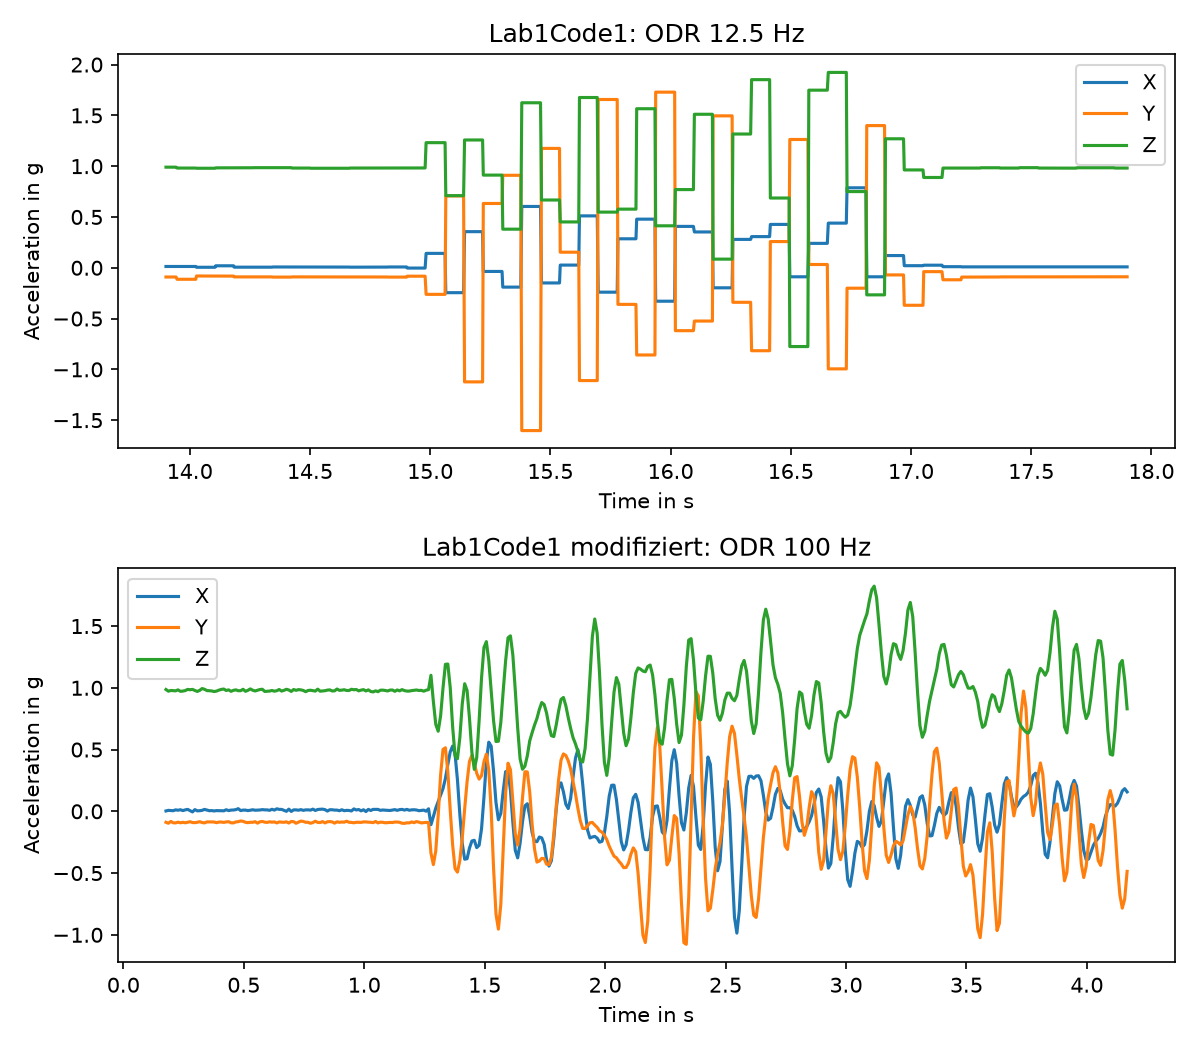
\includegraphics[width=0.72\textwidth]{A5_Vergleich_12_5Hz_100Hz.png}
  \caption{Comparison of 4\,s each: top A4 with ODR 12.5\,Hz (BMA400), bottom A5 with ODR 100\,Hz and $\pm 8\,g$ (MMA8452Q, modified code).}
  \label{fig:a5}
\end{figure}

\textbf{Comparison (Fig.~\ref{fig:a5}):} The measurement from Task~4 was recorded with the
BMA400 (ODR 12.5\,Hz), the new measurement with the MMA8452Q (ODR 100\,Hz);
since both are converted to $g$, the values are directly comparable. Both
share the rest level with a magnitude of approx.\ $1\,g$ in the $z$ direction ($x$ and
$y \approx 0$); in the new measurement the sensor was upside down, hence
$z \approx -1\,g$. At 100\,Hz there are no more steps: the curve is smooth
and the individual up-and-down movements (approx.\ 1--2 per second) are visible as an oscillation around
the rest level, whereas at 12.5\,Hz the signal is chopped up by aliasing.
The amplitudes are smaller in the new measurement (mostly
$\pm 0.5\,g$) because the movement was less vigorous. Isolated spikes down to approx.\
$-3\,g$ that last only one sample are probably impacts or outliers; thanks to
$\pm 8\,g$ they are not clipped. The essential difference is thus the
higher sampling rate.

\subsection{Time Stamp and Static Measurement in Six Orientations (Task 6)}

Each line receives the time stamp \texttt{millis()} directly on the Arduino
(4th column), independently of the time stamps of the serial monitor. From this, the mean
sampling frequency is calculated in Section~\ref{sec:fs}.

\textbf{(a)} Figure~\ref{fig:a6} shows the entire measurement.

\begin{figure}[H]
  \centering
  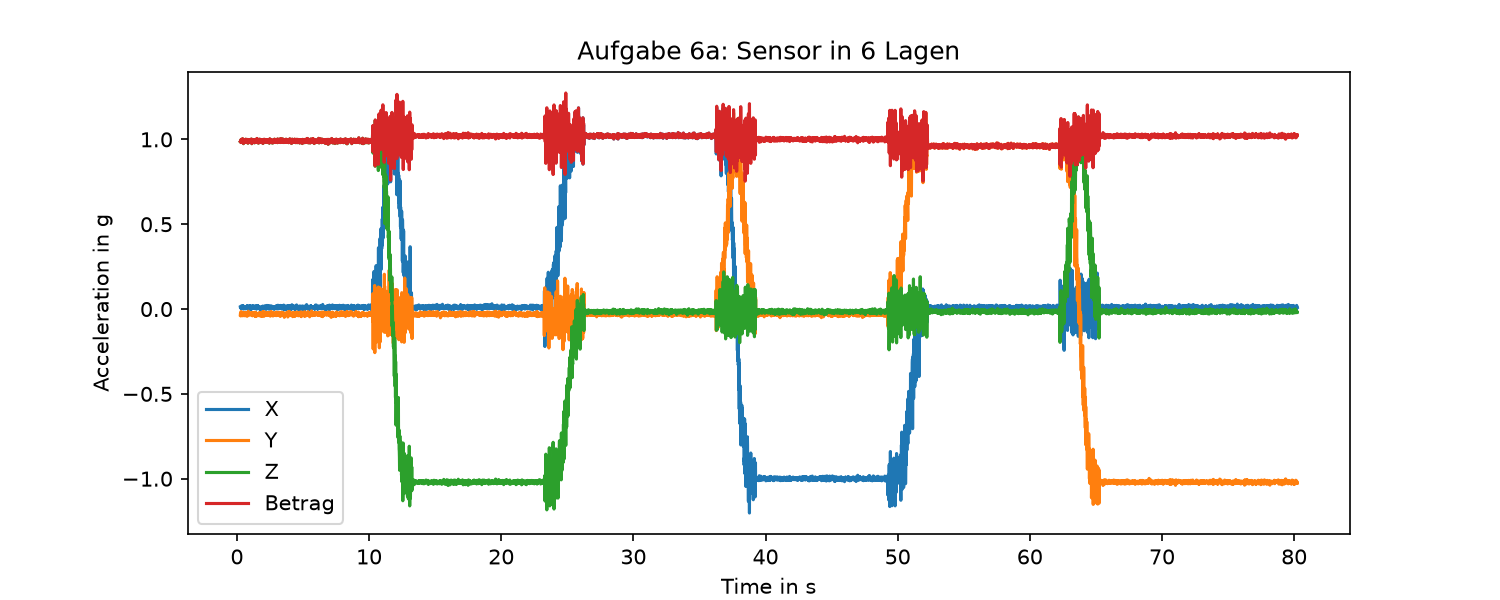
\includegraphics[width=0.9\textwidth]{A6a_6_Lagen.png}
  \caption{Sensor in six orientations of approx.\ 10\,s each; red: magnitude $|a| = \sqrt{x^2+y^2+z^2}$.}
  \label{fig:a6}
\end{figure}

\textbf{(b) Plausibility:} Table~\ref{tab:lagen} shows the mean values during the
rest phases.

\begin{table}[H]
\centering
\small
\caption{Mean acceleration in the six orientations (values in $g$).}
\label{tab:lagen}
\begin{tabular}{lcccc}
\toprule
Orientation & $x$ & $y$ & $z$ & $|a|$ \\
\midrule
$z$ up    & 0.01 & $-0.03$ & \textbf{0.99} & 0.99 \\
$z$ down  & 0.01 & $-0.03$ & \textbf{$-$1.02} & 1.02 \\
$x$ up    & \textbf{1.02} & $-0.03$ & $-0.02$ & 1.02 \\
$x$ down  & \textbf{$-$1.00} & $-0.03$ & $-0.02$ & 1.00 \\
$y$ up    & 0.01 & \textbf{0.96} & $-0.02$ & 0.96 \\
$y$ down  & 0.01 & \textbf{$-$1.02} & $-0.02$ & 1.02 \\
\bottomrule
\end{tabular}
\end{table}

The data make sense: the vertical axis always reads approx.\ $\pm 1\,g$,
the others approx.\ $0\,g$, and the magnitude is always approx.\ $1\,g$. If an axis points
upwards, the value is positive because the sensor measures the reaction force of the
supporting surface. The small deviations (up to 0.04\,$g$) result from offset errors
of the sensor and from the fact that it was not held exactly straight by hand.

\subsection{Filtering of the Data (Task 7)}

The data from Task~6 were filtered with a 4th-order Butterworth low-pass filter with a
cut-off frequency of $f_g = 5$\,Hz. For this, \texttt{filtfilt()} from
\texttt{scipy.signal} \cite{scipy} was used, which applies the filter forwards and backwards
and thus causes no phase shift (zero-phase filter).

\begin{figure}[H]
  \centering
  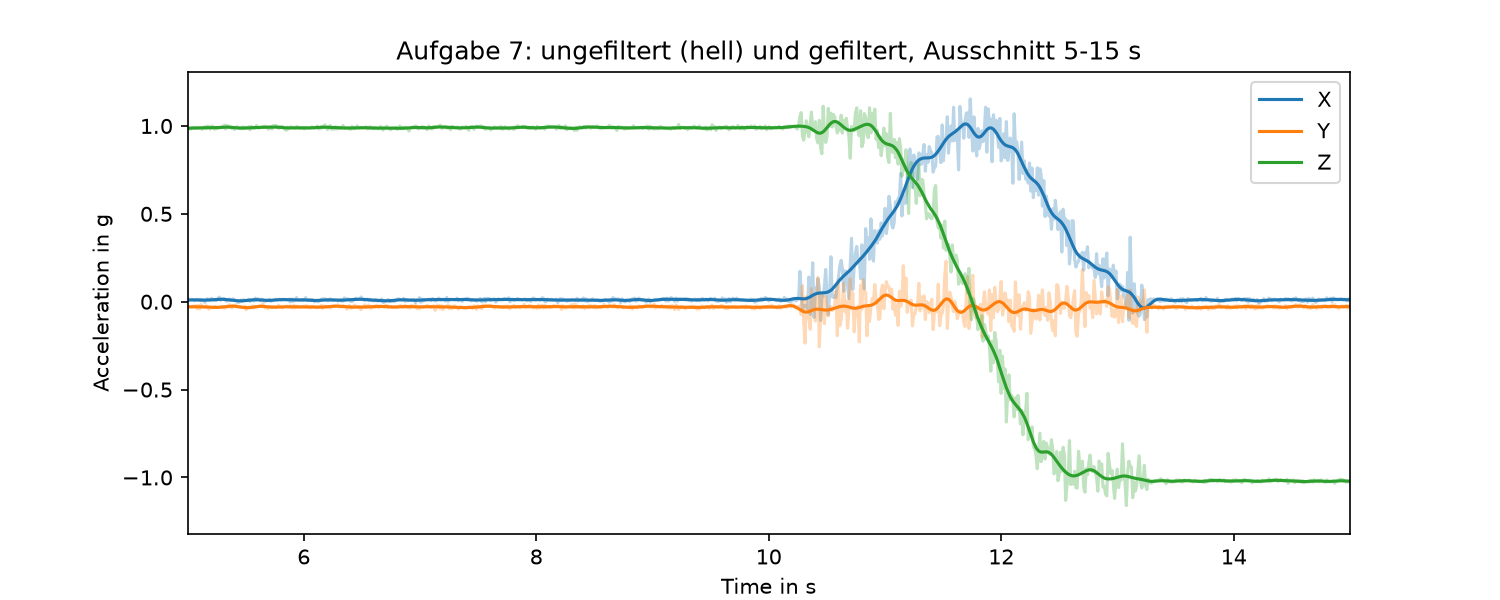
\includegraphics[width=0.9\textwidth]{A7_Filter.png}
  \caption{Unfiltered (light) and low-pass filtered data ($f_g = 5$\,Hz), excerpt 5--15\,s.}
  \label{fig:a7}
\end{figure}

\textbf{Effect and justification:} The filter removes sensor noise and hand
tremor (at rest, the standard deviation of $z$ drops from 6.0 to
1.6\,m$g$), while the changes of orientation are preserved and not shifted thanks to
\texttt{filtfilt} (Fig.~\ref{fig:a7}). A low-pass filter was chosen because the
orientation changes only slowly, whereas the noise is high-frequency.

\subsection{Determination of the Sampling Frequency (Task 8)}
\label{sec:fs}

From the \texttt{millis()} time stamps, the sampling intervals
$\Delta t_i = t_{i+1}-t_i$ and from them
\begin{equation}
  \bar f_s = \frac{1}{\overline{\Delta t}}, \qquad
  \sigma_{f_s} \approx \frac{\sigma_{\Delta t}}{\overline{\Delta t}^{\,2}}
\end{equation}
were determined (error propagation). Figure~\ref{fig:a8} shows the distribution of the
intervals, Tab.~\ref{tab:fs} the results.

\begin{figure}[H]
  \centering
  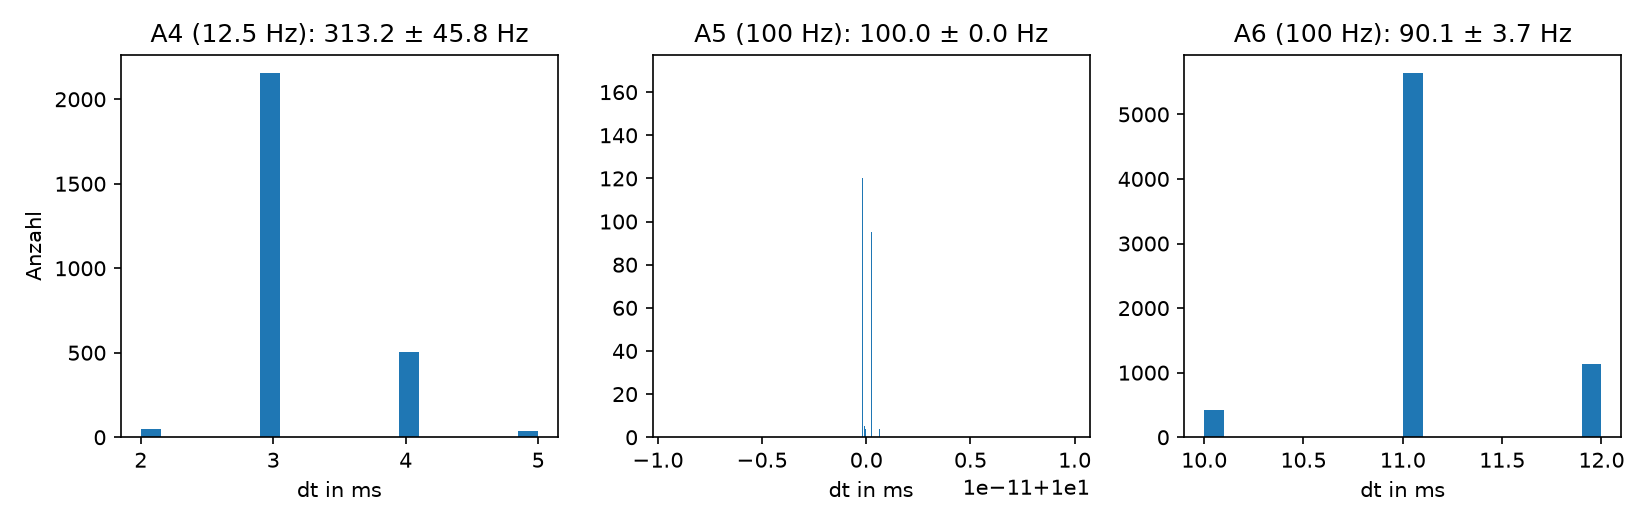
\includegraphics[width=\textwidth]{A8_Abtastfrequenz.png}
  \caption{Histograms of the sampling intervals $\Delta t$ of the three measurements.}
  \label{fig:a8}
\end{figure}

\begin{table}[H]
\centering
\small
\caption{Sampling intervals and sampling frequencies of the measurements.}
\label{tab:fs}
\begin{tabular}{lccc}
\toprule
Measurement & $\overline{\Delta t}$ / ms & $\sigma_{\Delta t}$ / ms & $\bar f_s$ / Hz \\
\midrule
A4: \texttt{Lab1Code1} (ODR 12.5\,Hz)          & 3.19  & 0.47 & $313 \pm 46$ \\
A5: modified (ODR 100\,Hz)                      & 9.91  & 0.65 & $100.9 \pm 6.6$ \\
A6: 6 orientations (ODR 100\,Hz)                & 11.10 & 0.46 & $90.1 \pm 3.7$ \\
A9: mobile system (\texttt{Lab1Code2})          & 18.79 & 0.95 & $53.2 \pm 2.7$ \\
\bottomrule
\end{tabular}
\end{table}

With \texttt{Lab1Code1} (A4), the loop without \texttt{delay} outputs at approx.\ 313\,Hz,
but new sensor values arrive only at 12.5\,Hz. In the modified code (A5),
output only occurs when there is a new sensor value (\texttt{available()}), so the clock
comes from the sensor: at $100.9 \pm 6.6$\,Hz, the sampling frequency matches the
configured ODR. That it is slightly above 100\,Hz is due to the tolerance of the sensor's
internal oscillator; the scatter (9--11\,ms) is mainly caused by
the 1\,ms resolution of \texttt{millis()}. In measurement A6 (BMA400, clocked via
\texttt{delay(10)}), by contrast, it is 90\,Hz, because the time for reading via
I\textsuperscript{2}C and for \texttt{Serial.print} is added to \texttt{delay(10)}
($\Delta t \approx 11$\,ms). Clocking via the sensor is therefore
more accurate. For a finer determination, \texttt{micros()} would be more suitable.

\subsection{Mobile Measurement System (Task 9)}

With the mobile measurement system (MMA8452Q, Qwiic OpenLog with SD card, battery),
545 values over 10.2\,s were recorded with \texttt{Lab1Code2}
(\texttt{IMU\_A9\_mobil\_Lab1Code2.txt}). The sensor lay mostly still and
slightly tilted; it was moved briefly only at approx.\ 2--3\,s. The mean
magnitude of the acceleration is $0.986\,g$, so the data are plausible
(Fig.~\ref{fig:a9}, left). The sampling frequency was determined as in Section~\ref{sec:fs}
and compared with the stationary measurement A6 (BMA400, ODR 100\,Hz, USB)
(Fig.~\ref{fig:a9}, right, and Tab.~\ref{tab:fs}). \texttt{Lab1Code2} already converts the raw values to $g$ (256\,LSB/$g$ at $\pm 8\,g$).

\begin{figure}[H]
  \centering
  \includegraphics[width=\textwidth]{A9_mobil.png}
  \caption{Mobile measurement system with \texttt{Lab1Code2}: left the measured data (10\,s),
  right the distribution of the sampling intervals compared with the stationary measurement A6.}
  \label{fig:a9}
\end{figure}

\textbf{Result:} The mobile system samples at
$\bar f_s = 53.2 \pm 2.7$\,Hz ($\overline{\Delta t} = 18.79 \pm 0.95$\,ms,
range 17--24\,ms), the stationary one at $90.1 \pm 3.7$\,Hz
($\overline{\Delta t} = 11.10 \pm 0.46$\,ms, range 10--12\,ms). The
mobile sampling frequency is thus approx.\ 40\,\% lower, and the absolute scatter of the intervals
is about twice as large, with isolated outliers up to 24\,ms.

\textbf{Discussion:} The sampling frequency is not determined by the sensor's ODR
but by the duration of one loop iteration on the microcontroller. In \texttt{Lab1Code2}, the
MMA8452Q runs at 200\,Hz, so only about every fourth
possible value is captured. In each iteration, the Arduino reads the status and $x$, $y$, $z$
individually via I\textsuperscript{2}C, calls \texttt{myLog.append()} (which reopens the
file for every value) and transmits the whole text line in five
\texttt{print} calls, also via I\textsuperscript{2}C, to the OpenLog. This
bus (standard 100\,kHz) is considerably slower than the serial output to the PC,
and the OpenLog additionally needs time to process the data and write them block-wise to
the SD card. This time varies, which is why the intervals scatter more and there are
isolated outliers up to 24\,ms. Furthermore, the setup differs as a whole:
a different sensor (MMA8452Q instead of BMA400), a different range ($\pm 8\,g$,
256\,LSB/$g$) and output with only two decimal places (resolution $0.01\,g$).
However, in both cases the time stamp and clock come from the Arduino (\texttt{millis()},
1\,ms resolution), so the sampling frequencies are directly comparable. Overall,
the slowest link in the signal chain determines the actual sampling frequency;
the ODR is only an upper limit.

% =====================================================================
\section{Summary}
% =====================================================================
The measurement system consisting of accelerometer (BMA400 or MMA8452Q), Arduino and PC
was set up and put into operation. With the default configuration (ODR
12.5\,Hz), the data did not represent the fast movement correctly because of the too low sampling rate
(aliasing) and repeatedly output values. By increasing the ODR
to 100\,Hz (\texttt{CTRL\_REG1} of the MMA8452Q) and the range to $\pm 8\,g$,
the movement was captured correctly (sampling frequency $100.9 \pm 6.6$\,Hz). The static measurement
confirmed an acceleration of approx.\ $1\,g$ in all six orientations (deviation
$\leq 0.04\,g$). A Butterworth low-pass filter (5\,Hz, \texttt{filtfilt}) reduced the
noise considerably without phase shift. The actual sampling frequency was
approx.\ 90\,Hz (stationary) and 53\,Hz (mobile, \texttt{Lab1Code2} with data logger).

% References: formatted as IEEEtran output for Literatur.bib, notes in English
\begin{thebibliography}{1}
\providecommand{\url}[1]{#1}
\providecommand{\newblock}{\relax}

\bibitem{sparkfun}
{SparkFun Electronics}, ``{SparkFun Triple Axis Accelerometer Breakout --
  BMA400 (Qwiic): Hookup Guide},'' Online.

\bibitem{bma400}
{Bosch Sensortec}, \emph{{BMA400 -- Ultra-low power triaxial accelerometer}},
  Bosch Sensortec GmbH, Reutlingen, data sheet, Rev.~2.3.

\bibitem{scipy}
P.~Virtanen \emph{et~al.}, ``{SciPy 1.0: Fundamental algorithms for scientific
  computing in Python},'' \emph{Nature Methods}, vol.~17, pp. 261--272, 2020.

\bibitem{mma8452q}
{NXP Semiconductors}, \emph{{MMA8452Q -- 3-axis, 12-bit/8-bit digital
  accelerometer}}, Freescale Semiconductor (now NXP), data sheet, Rev.~8.1.

\end{thebibliography}

\textbf{Note on the use of AI:} AI tools (Claude, Anthropic) were used in preparing this report and the
Python code as aids for wording texts as well as for code and debugging. All measurements
were carried out by the group itself; results and content were checked by the group.

% =====================================================================
\appendix
\section{Appendix: Submitted Files (Task 10)}
\label{sec:anhang}
% =====================================================================
The submission \texttt{Lab1\_Gruppe\_4.zip} contains:
\begin{itemize}
  \item \texttt{Bericht\_1\_Gruppe\_4.pdf} -- this report,
  \item \texttt{Lab1Code1\_modifiziert.ino} -- modified Arduino code (Task 5),
  \item \texttt{MainCode1.ipynb} -- Python evaluation (Tasks 4a, 5, 6a, 7, 8, 9); runs completely and saves all figures in \texttt{figures/},
  \item data sets in \texttt{data/}: \texttt{IMU\_A4\_Lab1Code1\_roh.csv}, \texttt{IMU\_A5\_Lab1Code1mod\_100Hz.csv}, \texttt{IMU\_A6\_Lagen.csv}, \texttt{IMU\_A9\_mobil\_Lab1Code2.txt}.
\end{itemize}

\end{document}
